%%%%%%%%%%%%%%%%%%%%%%%%%%%%%%%%%%%%%%%%%

%----------------------------------------------------------------------------------------
%	PACKAGES AND OTHER DOCUMENT CONFIGURATIONS
%----------------------------------------------------------------------------------------

\documentclass[a4paper,10pt]{article}

\usepackage[utf8]{inputenc} % Required for inputting international characters
\usepackage[T1]{fontenc} % Output font encoding for international characters
% !TEX encoding = UTF-8 Unicode
%\usepackage[utf8]{inputenc}
\usepackage{pdfpages}
\usepackage{mathtools}
\usepackage{amsmath}
\usepackage{fullpage}
\usepackage{bm}
\usepackage{float}
\usepackage{gensymb}
\graphicspath{./dir/} 
\usepackage{mathpazo} % Palatino font


\begin{document}

%----------------------------------------------------------------------------------------
%	TITLE PAGE
%----------------------------------------------------------------------------------------

\begin{titlepage} % Suppresses displaying the page number on the title page and the subsequent page counts as page 1
	\newcommand{\HRule}{\rule{\linewidth}{0.5mm}} % Defines a new command for horizontal lines, change thickness here
	
	\center % Centre everything on the page
	
	%------------------------------------------------
	%	Headings
	%------------------------------------------------

	
	\textsc{\LARGE University of Oslo}\\[1.5cm] % Main heading such as the name of your university/college
	
	\textsc{\Large Control of Mobile Robots}\\[0.5cm] % Major heading such as course name
	
	\textsc{\large UNIK4490}\\[0.5cm] % Minor heading such as course title
	
	%------------------------------------------------
	%	Title
	%------------------------------------------------
	
	\HRule\\[0.4cm]
	
	{\huge\bfseries Odometry and Posture Regulation for a 4 by 4 mobile robot}\\[0.4cm] % Title of your document
	\HRule\\[0.8cm]
	{\large{Autumn 2017}} % Date, change the \today to a set date if you want to be precise	
	\vspace{1cm}
	%------------------------------------------------
	%	Author(s)
	%------------------------------------------------
	
	\begin{minipage}{0.4\textwidth}
		\begin{flushleft}
			\large
			\textit{Authors}\\
			Eirik \textsc{Kvalheim}, Daniel \textsc{Sander Isaksen} and Torgrim \textsc{R. Næss}
		\end{flushleft}
	\end{minipage}
	~
	\begin{minipage}{0.4\textwidth}
		\begin{flushright}
			\large
			\textit{Supervisors}\\
			Dr. Kim \textsc{Mathiassen} and Magnus \textsc{Baksaas}
		\end{flushright}
	\end{minipage}
	
	% If you don't want a supervisor, uncomment the two lines below and comment the code above
	%{\large\textit{Author}}\\
	%John \textsc{Smith} % Your name
	
	%------------------------------------------------
	%	Date
	%------------------------------------------------
	
	\vfill\vfill\vfill\vfill\vfill\vfill\vfill\vfill\vfill\vfill\vfill\vfil\vfill\vfill\vfill\vfill\vfill\vfill\vfill\vfill\vfill\vfill\vfill\vfill\vfill\vfill\vfill\vfill%  go wild
	
	
	%------------------------------------------------
	%	Logo
	%------------------------------------------------
	
	%\vfill\vfill
	%\includegraphics[width=0.2\textwidth]{placeholder.jpg}\\[1cm] % Include a department/university logo - this will require the graphicx package
	\begin{figure}[H]
	\raggedright
	 
\includegraphics[width=0.15\textwidth]{uiologo.png}
	\end{figure}
	 
	%----------------------------------------------------------------------------------------
	
	\vfill % Push the date up 1/4 of the remaining page
	
\end{titlepage}

%----------------------------------------------------------------------------------------


\renewcommand{\labelenumi}{\alph{enumi})}


	\begin{figure}[H]
	\centering
	 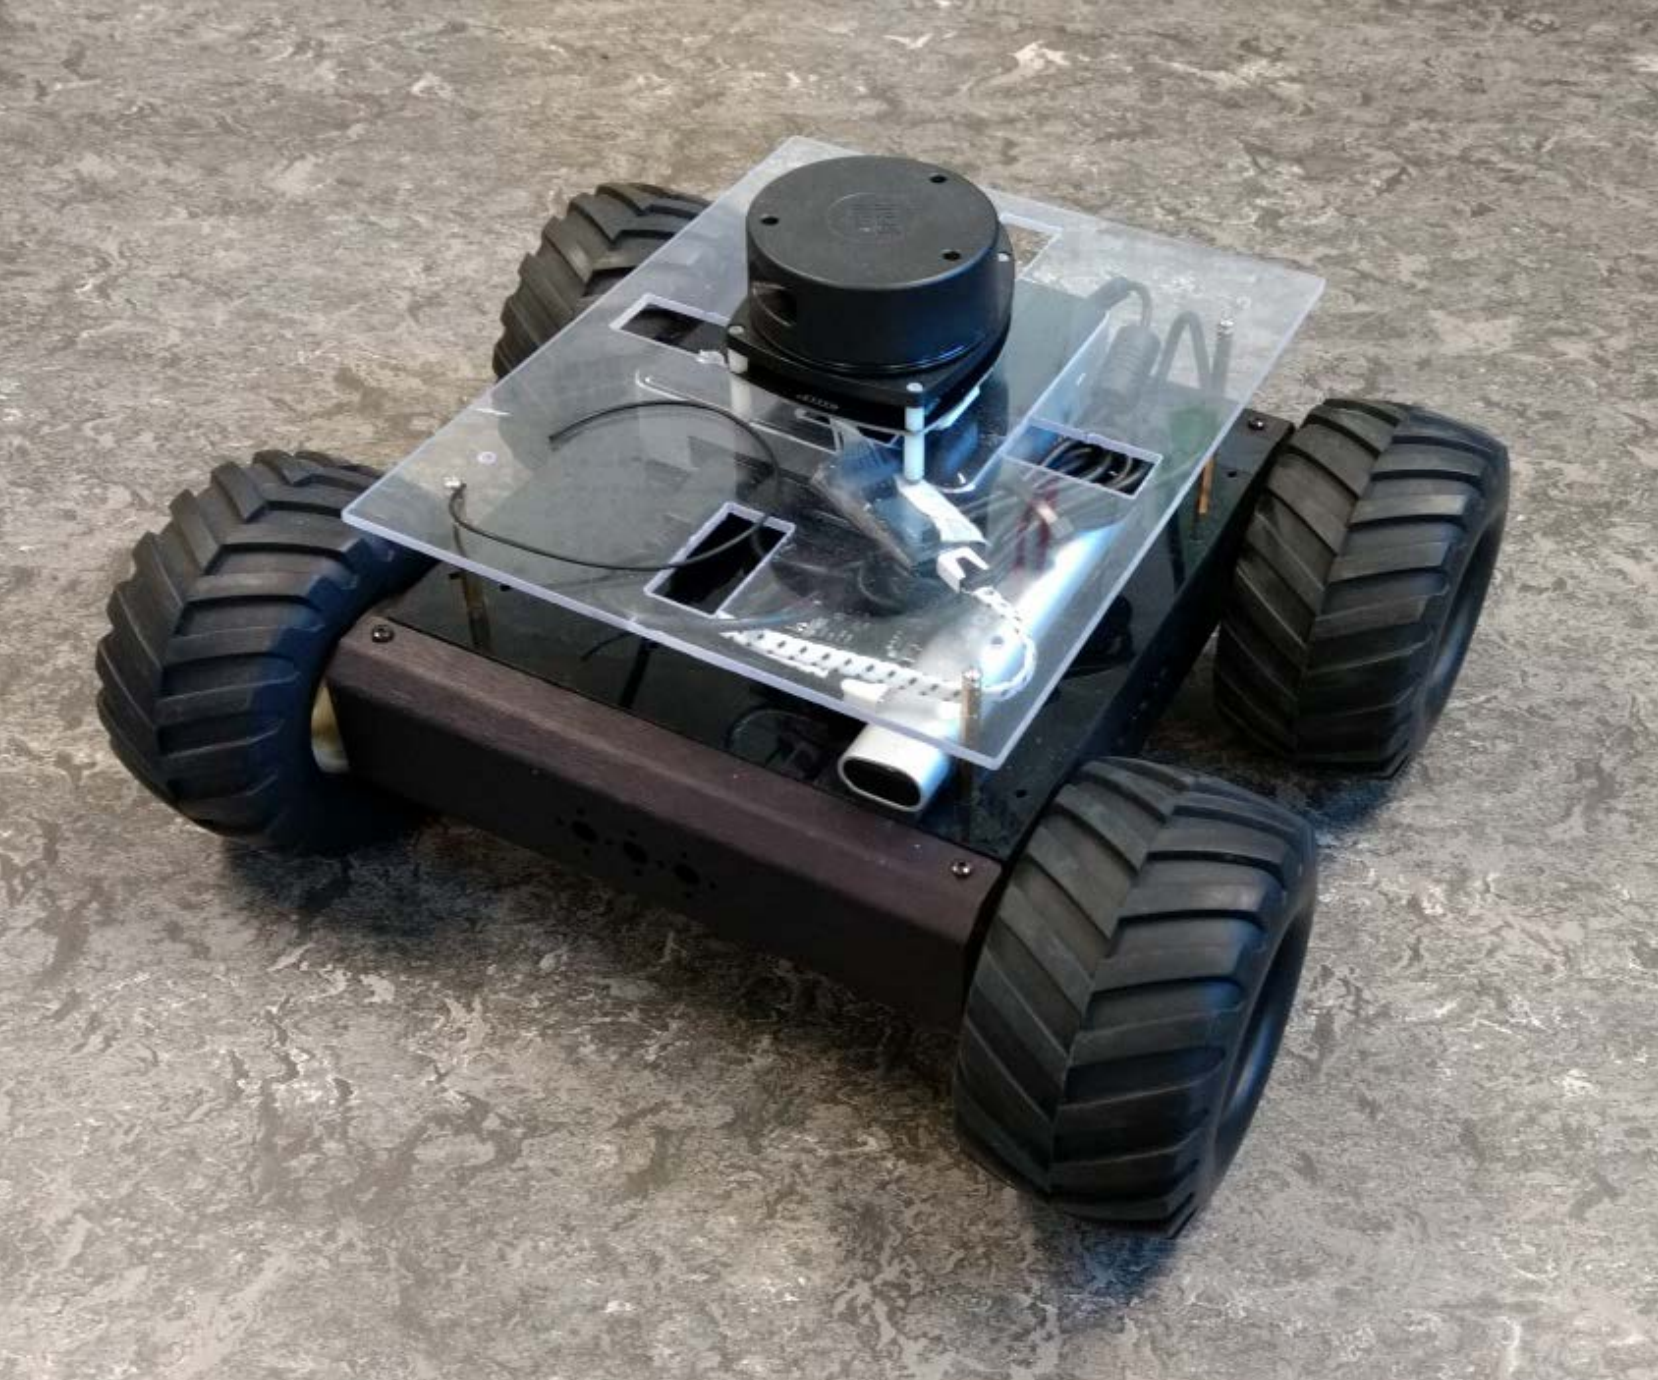
\includegraphics[width=0.5\textwidth]{rover_pic.png}
	%\caption{Rover}	
 	%\label{fig:1}
	\end{figure}

\section{Introduction}
The main goal of this project was to implement motor control, posture regulation and odometric localization in order to get the robot to move to a desired pose. We were working on an existing software stack running ROS (Robot Operating System), so getting to know the previous software aswell as ROS as a system, was also a goal in this project.\\
A significant portion of the project time was spent on reverse engineering the robot to better understand the system in order to implement our own solutions. In the end we had also spent a lot of time on tuning the regulator parameters, aswell as compensating for odometric faulties. Most of the work was done in collaboration with another group that were working on an identical robot with the same software stack. \\

\section{The System}
Figure 1 illustrates our implementation of the system with control loop. It consists of posture regulaton, motor controller, kinematic model, and odometry. Here we are setting a desired pose, and the posture regulator tries to drive the error towards 0.

	\begin{figure}[H]
	\centering
	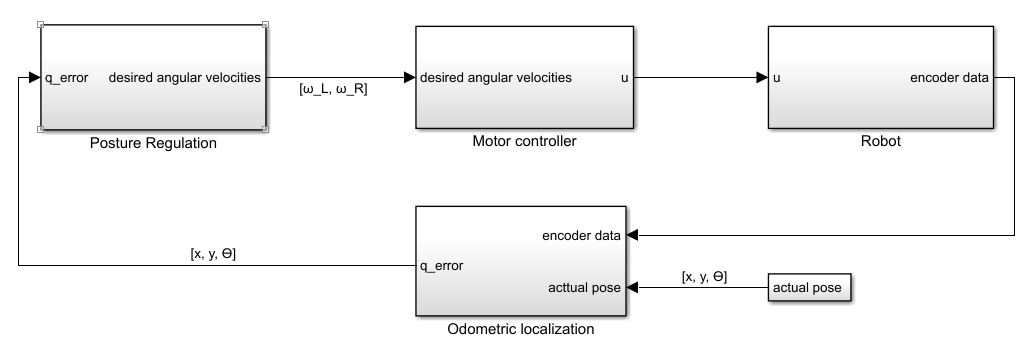
\includegraphics[width=0.9\textwidth]{blokkskjema.JPG}
	\caption{System with Control loop}	
 	\label{fig:2}
	\end{figure}

\subsection{Kinematic Model}
We used the kinematic model of a unicycle derived in chapter 11.2.1 in "Robotics - Modelling, Planning and Control" by B. Siciliano et.al. Here $v$ is the driving velocity and $\omega$ is the steering velocity.

\begin{equation}
	\begin{bmatrix}
	\dot{x}\\ 
	\dot{y}\\
	\dot{\theta}\\  
	\end{bmatrix}
	=
	\begin{bmatrix}
	cos\theta\\ 
	sin\theta\\
	0\\  
	\end{bmatrix}v
	+
	\begin{bmatrix}
	0\\ 
	0\\
	1\\  
	\end{bmatrix}\omega
\end{equation}


...the driving and steering velocities $v$ and $omega$ are expressed as a function of the actual velocity inputs, i.e., the angular speeds $\omega_{R}$ and $\omega_{L}$ of the right and left wheels, respectively:

		\begin{equation}
			v=\frac{r(\omega_R +\omega_L)}{2}
		\end{equation}

		\begin{equation}
			\omega=\frac{r(\omega_R -\omega_L)}{d}
		\end{equation}


\subsection{Motor Control}
	The implementation of motor control for each wheel was already available in the software stack. We started our project by reverse engineering the code in order to get the motor driver to work.
This motordriver/controller had an internal pid regulator, and uses encoder data to calculate wheel velocities.
	As we were not familiar with the system, and since there were no documentation or comments in the code, we faced challenges on elementary problems as; communication with the robot, running the motordriver and deducing the reason behind the constants in the controller.
In the end it turned out that there was an usb port which needed to be taken in and out every time the motordriver runs the first time. This was the usb connecting the teensy that reads the encoders. There are still unknown constants in this code that has an effect on the published velocity, so we cannot know if this motordriver is publishing correct speeds or not. We ended up assuming that it was correct and moved on to derive the odometry and posture regulator.
	

\subsection{Odometric Localization}

		The implementation of any feedback controller requires the availability of the robot configuration at each time instant. Since we are not using any external sensors for doing SLAM
		(Simultaneous Localization And Mapping), our only sensors for knowing where we are is the encoders located on each wheel. In order to use this information to know where we are located
		and heading (in a world/reference coordinate frame), we need to calculate the \emph{Odometry}. The method used is odometry by exact integration, and can be found in chapter 11.7 in
		"Robotics - Modelling, Planning and Control" by B. Siciliano et.al. Here we obtain the following equations in chained form:
		
		\begin{equation}
		x_{k+1}=x_k+\frac{v_k}{\omega_k}(sin\theta_{k+1}-sin\theta_k)
		\end{equation}
		\begin{equation}
		y_{k+1}=y_k+\frac{v_k}{\omega_k}(cos\theta_{k+1}-cos\theta_k)
		\end{equation}
		\begin{equation}
		\theta_{k+1}=\theta_k+\omega_kT_s
		\end{equation}
		
		Where $\theta_{k+1}$ is the angle for the next time step relative to the reference frame, $T_s$ is the time step, and $x_{k+1}$ and $y_{k+1}$ are the Cartesian position of the robot for
		the next time step, relative to the reference frame.

		$v_k$ and $\omega_k$ is obtained by equation (2) and (3), and thus giving us the complete odometry. The angular velocities $\omega_R$  and $\omega_L$ is obtained by subscribing to
		the topic \textit{/est\_vel} which is published from the motordriver.\\

		We initialize our odometry node by calculating where our robot is in the reference frame, and sending these variables as an input to the node. Assuming perfect posture control, the robot will
		then move towards zero position in the reference frame. One case could look like this;


		\begin{figure}[H]
		\centering
		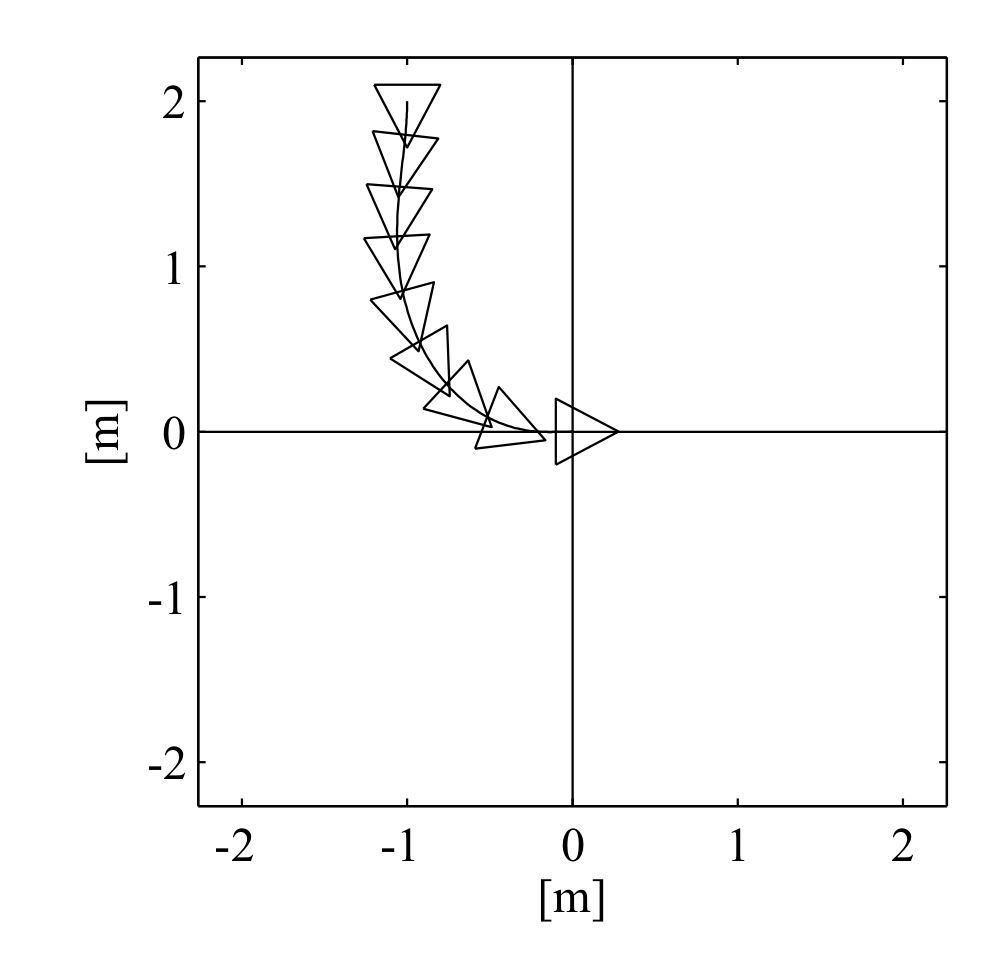
\includegraphics[width=0.4\textwidth]{odometric_localization_config.JPG}
		\caption{Localization from start to finish}	
 		%\label{fig:2}
		\end{figure}



		
\subsection{Posture Regulation}

	
		We have implemented posture control from chapter 11.6.2 in  "Robotics - Modelling, Planning and Control" by B. Siciliano et.al. 
		In general the posture regulation controller takes in the configuration vector $q = [x, y, \theta]^{T}$ (Cartesian position and vehicle orientation), 
		and outputs v and $\omega$. We obtain the input vector $q$ by subscribing to the topics \textit{/odometry} and \textit{/theta}, published by the odometry.
		It is assumed that the desired variables are $q_{d} = [0, 0, 0]^{T}$ and the error from $q_{d}$ is represented by
		\begin{equation}
			\rho = \sqrt{x^{2} + y^{2}} 
		\end{equation}
		\begin{equation}
			\gamma = Atan2(y, x) - \theta + \pi
		\end{equation}
		\begin{equation}
			\delta = \gamma + \theta
		\end{equation}
		where $\rho = ||\vec{e_{p}}||$ is the distance between current point $(x, y)$ and desired point $(0, 0)$, 
		$\gamma$ is the angle between $\vec{e_{p}}$	and the sagittal axis of the vehicle and $\delta$ is the axis between $\vec{e_{p}}$ and the x-axis.	
		v and $\omega$ are found by:
		\begin{equation}
			v = k_{1}\rho cos(\gamma)
		\end{equation}		
		\begin{equation}
			\omega = k_{2}\gamma + k_{1}\frac{sin(\gamma)cos(\gamma)}{\gamma}(\gamma + k_{3}\delta)
		\end{equation}
		
		In our implementation of the controller we get $\vec{q}$ from the odometric module and output $\omega_{R}$ and $\omega_{L}$ to the motor controller. 
		This is done by publishing the angular velocities to the topic \textit{/cmd\_vel}, which the motordriver subscribes on in order to control the velocities.
		Equations for $\omega_{R}$ and $\omega_{L}$ expressed by error variables $\rho$, $\gamma$ and $\delta$, can be found
		by setting equation (2) and (3) equal to equation (10) and (11), and then solving for $\omega_{R}$ and $\omega_{L}$. This yields:		
		\begin{equation}
			\omega_{R} = \frac{2k_{1}\rho cos(\gamma)}{2r} + \frac{k_{2}d\gamma}{2r} + \frac{k_{1}dsin(\gamma)cos(\gamma)(\gamma + k_{3}\delta)}{2r\gamma}
		\end{equation}
		\begin{equation}
			\omega_{L} = \frac{2k_{1}\rho cos(\gamma)}{2r} - \frac{k_{2}d\gamma}{2r} - \frac{k_{1}dsin(\gamma)cos(\gamma)(\gamma + k_{3}\delta)}{2r\gamma}
		\end{equation}

		Where $d$ is the distance between the outer gripping point of the wheels (almost width of the rover), and $k_{1}$, $k_{2}$ and $k_{3}$ are the controller gains.
		It is woth noting that in equation (6) we are using atan2, which is a function that is undefined in $x=y=0$, therefore $\gamma$ and $\delta$ is also undefined for $x=y=0$.
		To avoid this problem we designed the controller to accept the position and orientation if each element of $q$ had less then 0.05 error. At first, while trying to adjust controller gains 
		we also tried to modify the controller further than the litterature did, to account for the weaknesses. We had no luck with this and ended up with implementing exactly the controller
		derived from the litterature. The funny thing was that we later understood that the controller already were proven asymptotically stable given the lyapunov candidate function

		\begin{equation}
			V = \frac{1}{2}(\rho^2 + \gamma^2 + k_{3}\delta^2)
		\end{equation}

		wihich yiealds the time derivative

		\begin{equation}
			\dot{V} = - k_{1}cos^2(\gamma)\rho^2 - k_{2}\gamma^2)
		\end{equation}

		where $\dot{V}$ is negative semi-definite. Further analysis of the closed-loop system leads to conclude that the system trajectory for the equilibrium posture is also tending to 0, 
		and thus the controller is stable.


\section{Testing, Results and Conclutions}

		After implementing the system and getting the ROS nodes to communicate, our system looked like this;

		\begin{figure}[H]
		\centering
		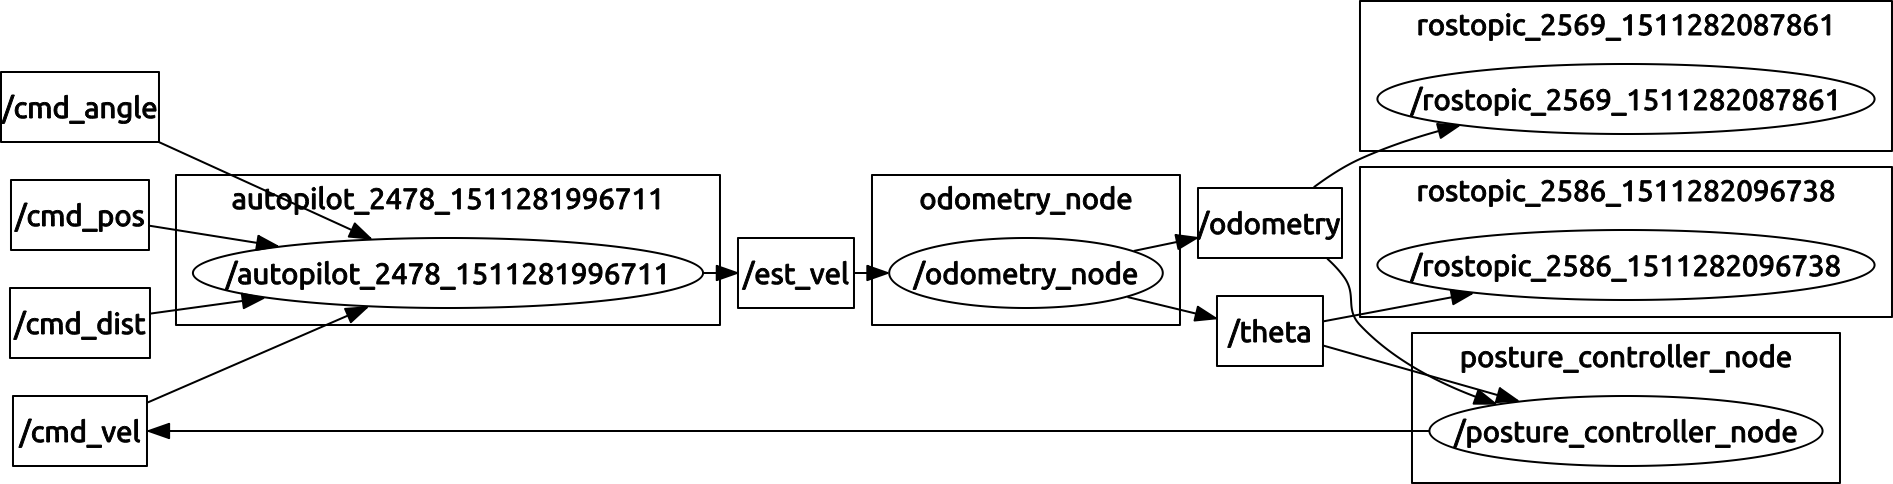
\includegraphics[width=0.9\textwidth]{rover2_rqt_graph.png}
		%\caption{code}	
 		%\label{fig:3}
		\end{figure}

		And as expected one can see assemblance to figure 1. Here you can see the motordriver labled as the node \textit{/autopilot}. \\


		We started by implementing the reccomended gains from the litterature, where $k_{1}=1$, $k_{2}=2.5$, and $k_{3}=3$, but hese gains did not provide a good regulator.
		Reflecting on the equations (8-13) and discussing which gains we needed to increase with regards to how the robot behaved, we came up with  $k_{1}=2$, $k_{2}=2.3$, and $k_{3}=1.3$
		wich was a pretty good regulator, with only a small accuracy problem. Increasing to $k_{1}=2$, $k_{2}=4$, and $k_{3}=1.3$ provided an even more accurate regulator, which
		conviniently happend to also be quicker.\\
		We also found another set of gains where $k_{1}=1$, $k_{2}=6$, and $k_{3}=7$ that gave a very slow and steady regulator, with very good accuracy at distances < 2m. Over 2m the
		"2 4 1.3" regulator was clearly better on minimizing the error.
		
		Blelow is a plot of the "2 4 1.3" regulator;
		\begin{figure}[H]
		\raggedleft
		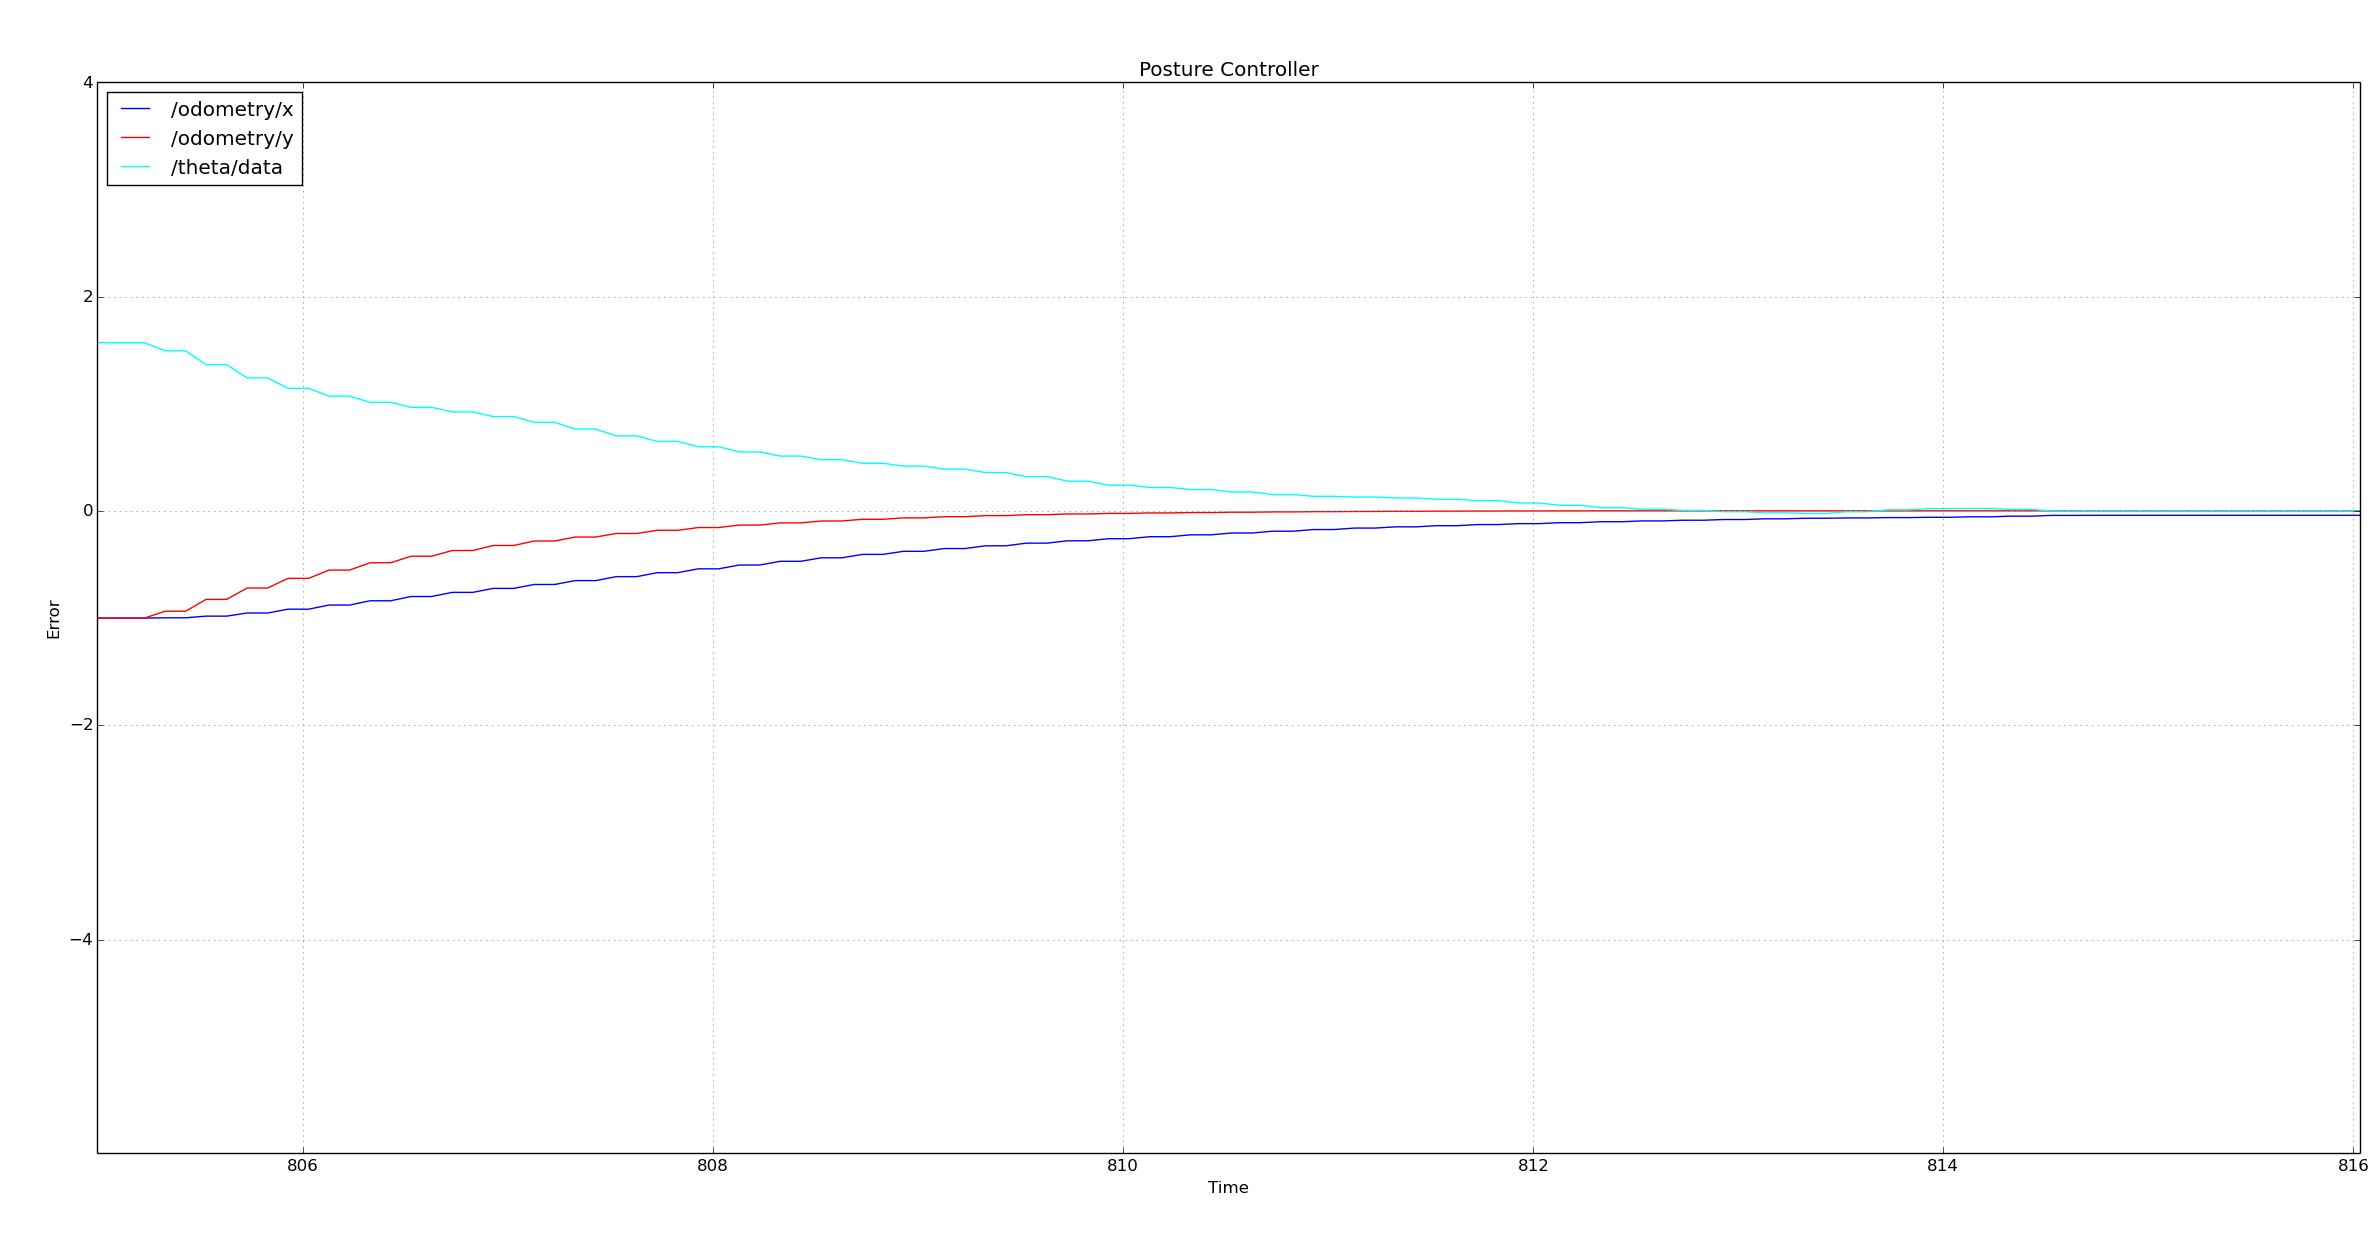
\includegraphics[width=1.1\textwidth]{rover2_rqt_plot94_2413.png}
		\caption{Regulator with gains $k_{1}=2$, $k_{2}=4$, and $k_{3}=1.3$}	
 		\label{fig:33}
		\end{figure}				 
	
		Where x and y starting position was -1m, and the robot started in $\theta=\frac{\pi}{2}$. Below is the exact same starting conditions for the "1 6 7" regulator;

		\begin{figure}[H]
		\centering
		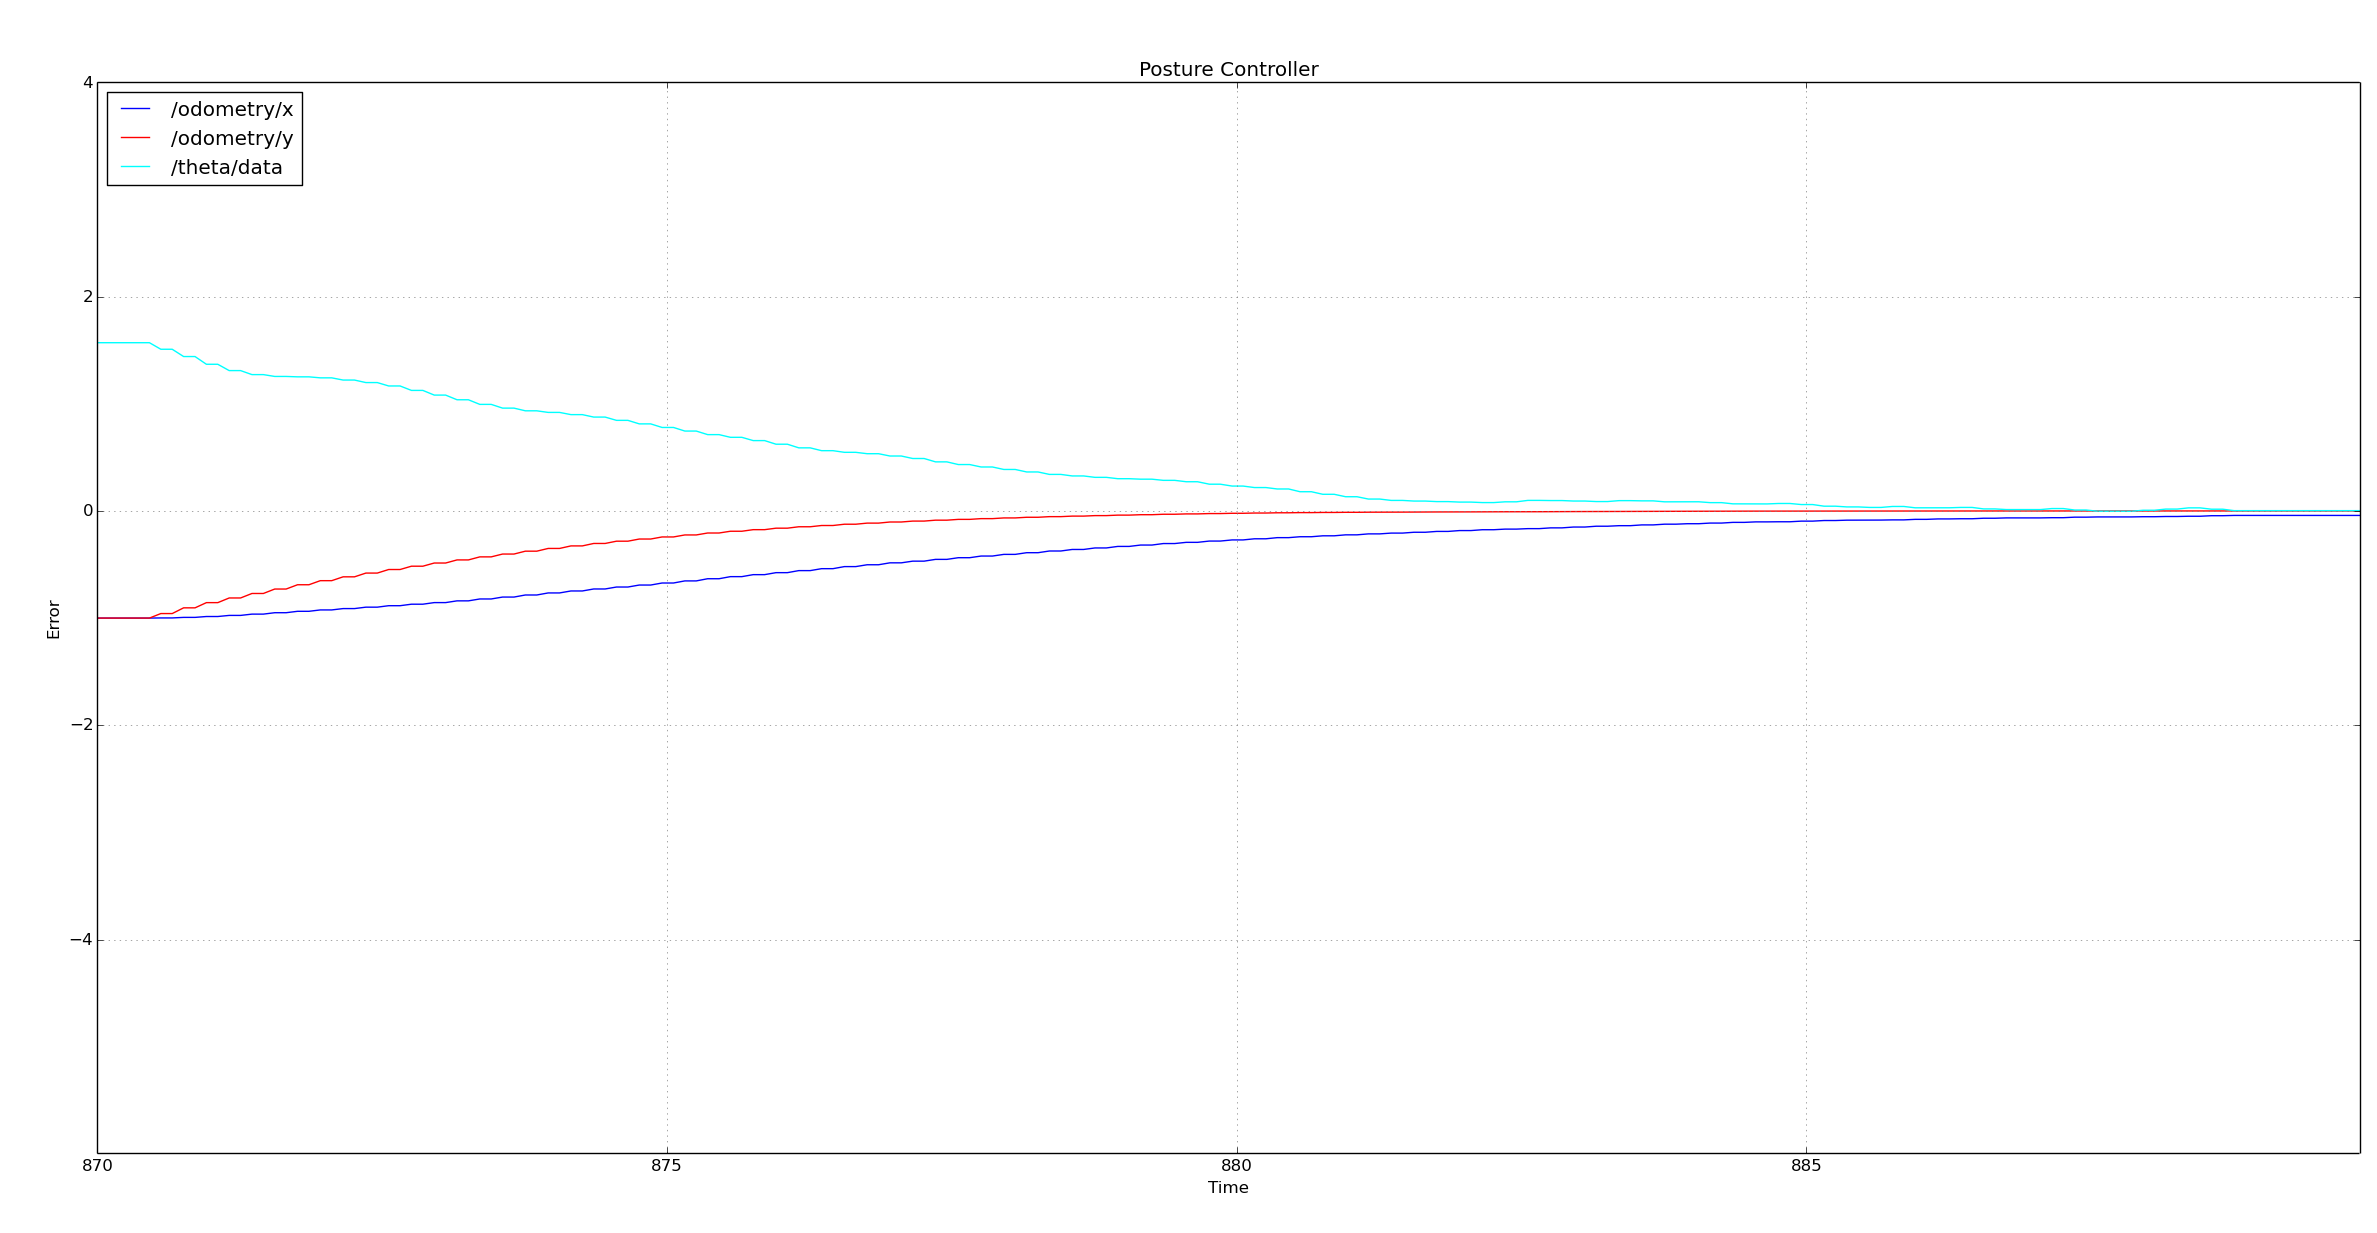
\includegraphics[width=1.1\textwidth]{rover2_rqt_plot94_167.png}
		\caption{Regulator with gains $k_{1}=1$, $k_{2}=6$, and $k_{3}=7$}
 		\label{fig:333}
		\end{figure}

		We can see that the "1 6 7" regulator (in the same case) uses approximately 10 seconds longer, but achieves the same goal.\\

		We concluded that the "2 4 1.3" regulator was the best one overall, and tested it further on other starting positions;

		%\begin{figure}[H]
		%\centering
		%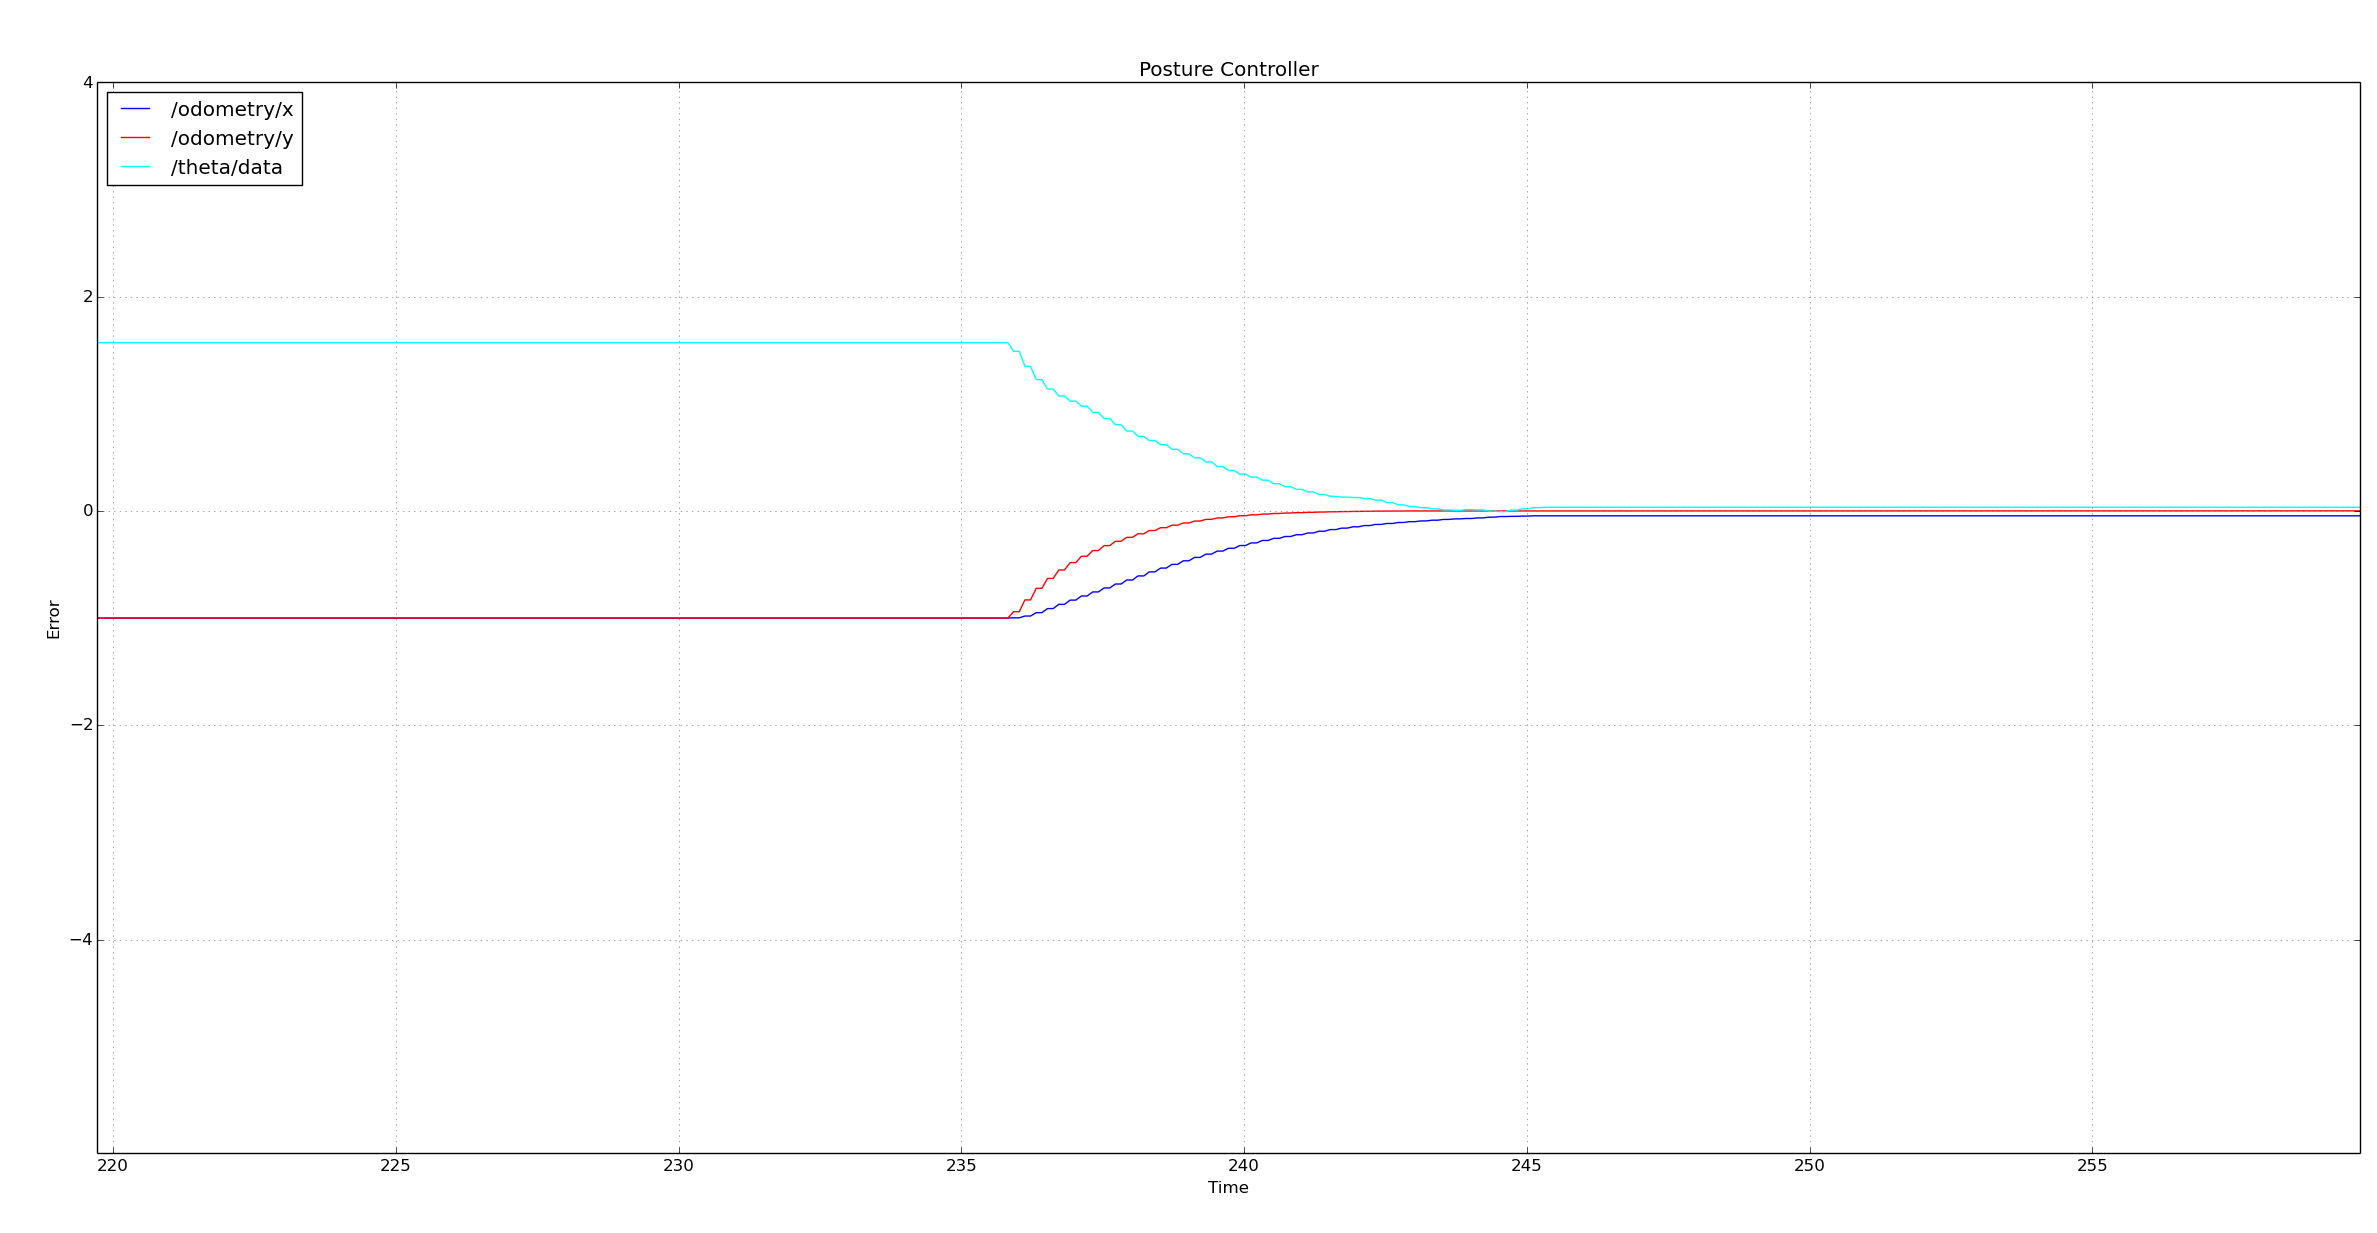
\includegraphics[width=1.1\textwidth]{rover2_rqt_plot9_0.png}
		%\caption{ $x = -1,  y = -1,  \theta=\frac{\pi}{2}$}	
 		%\label{fig:3232}
		%\end{figure}


		\begin{figure}[H]
		\centering
		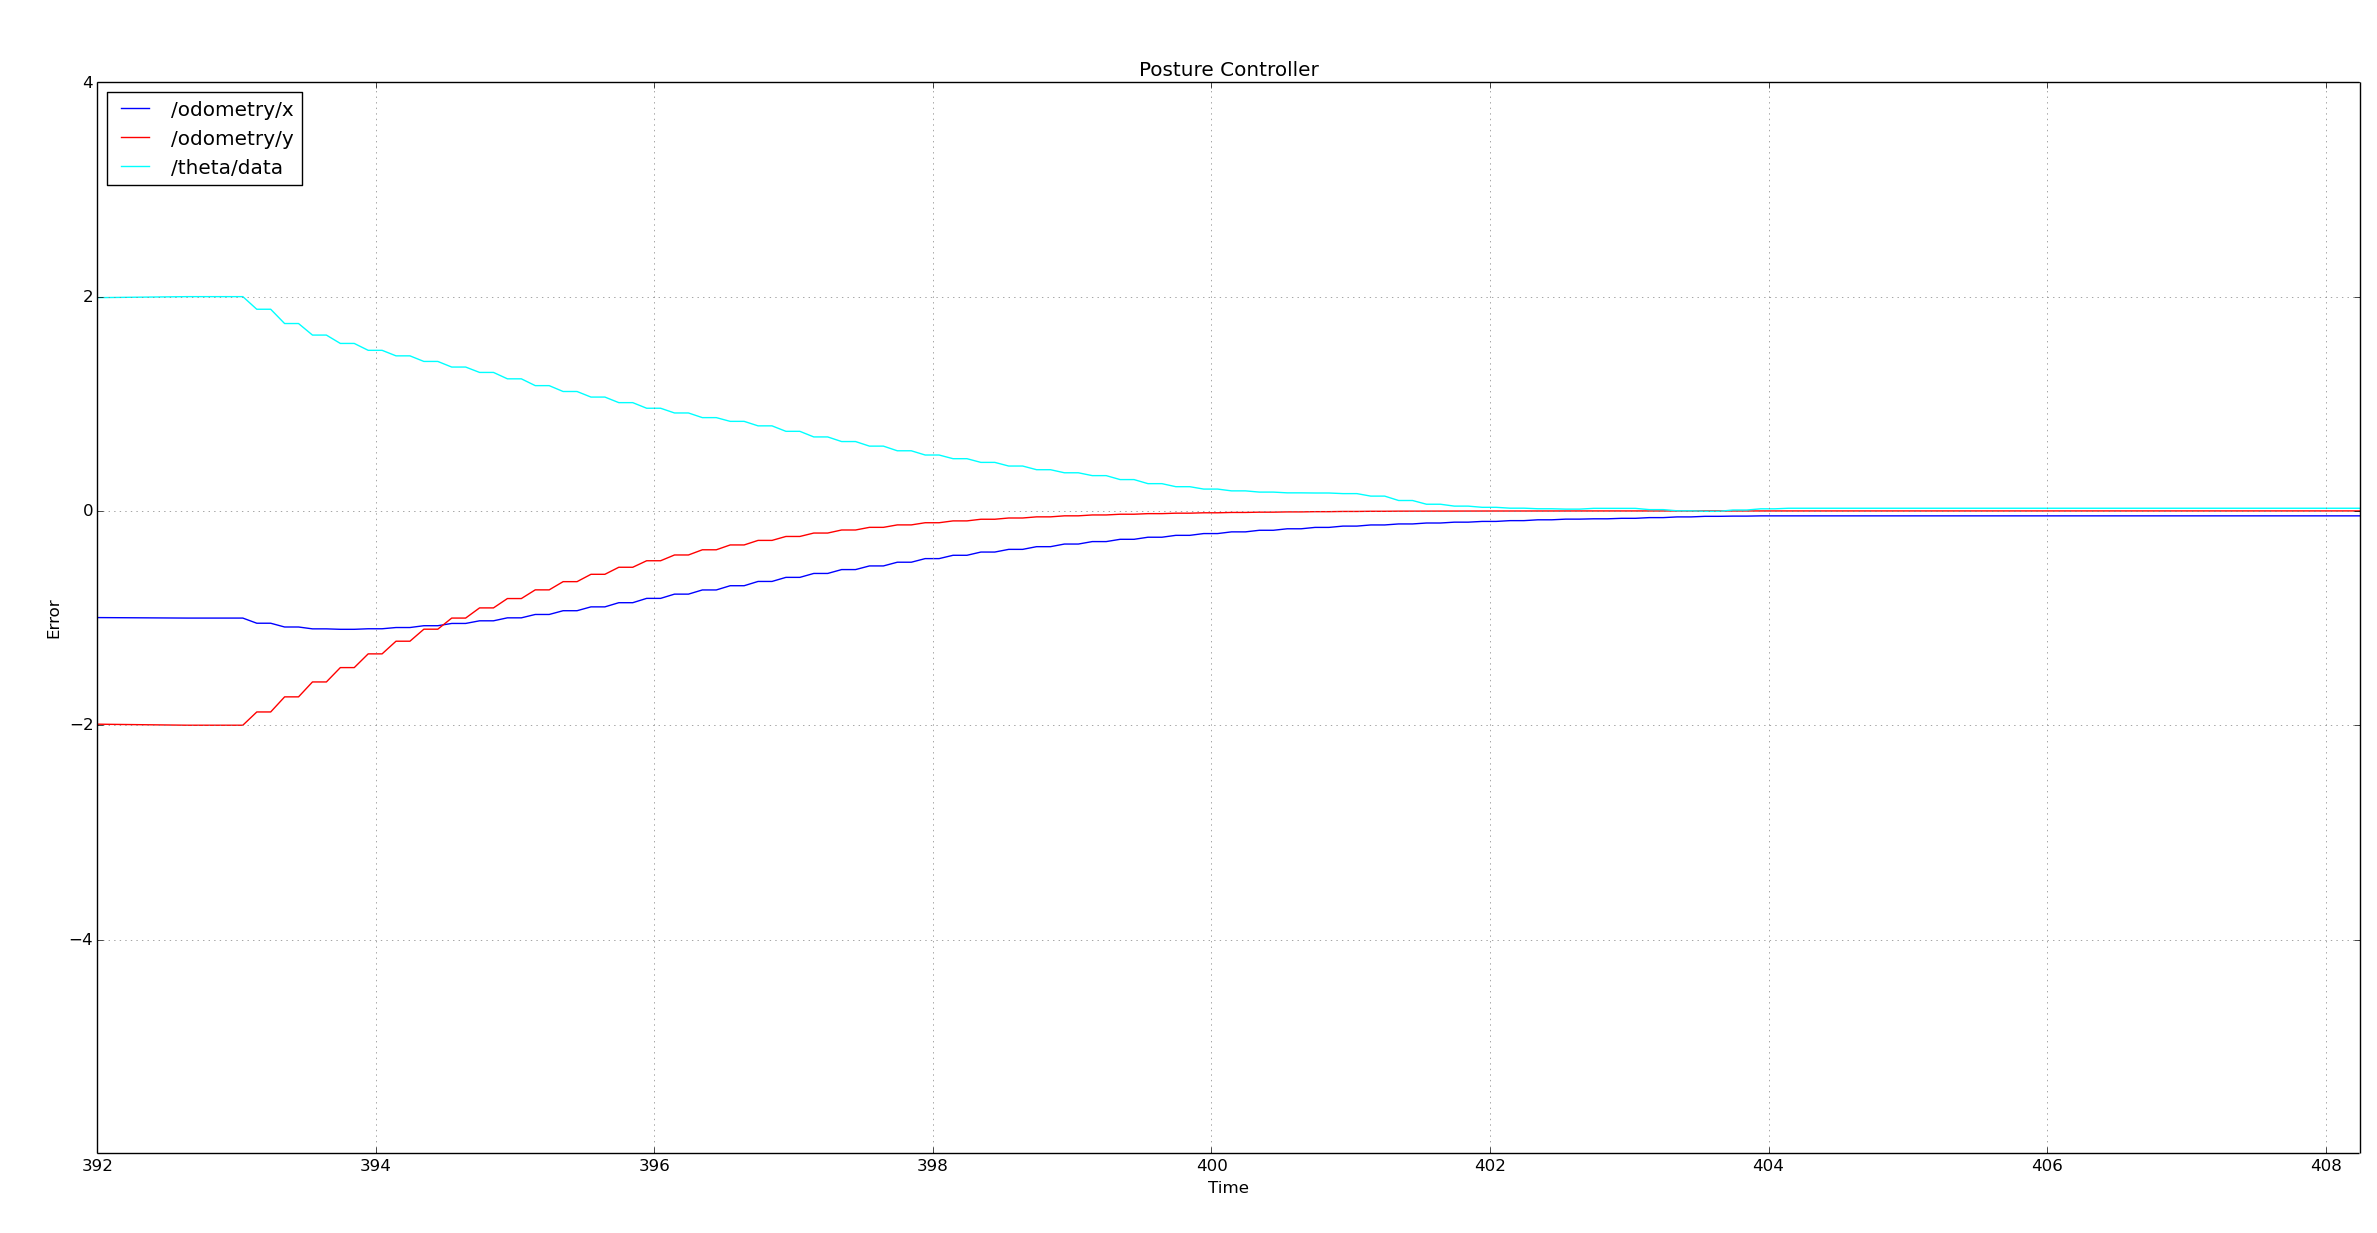
\includegraphics[width=1.1\textwidth]{rover2_rqt_plot91.png}
		\caption{ $x = -1,  y = -2,  \theta = 2$}	
 		\label{fig:35657}
		\end{figure}



		\begin{figure}[H]
		\centering
		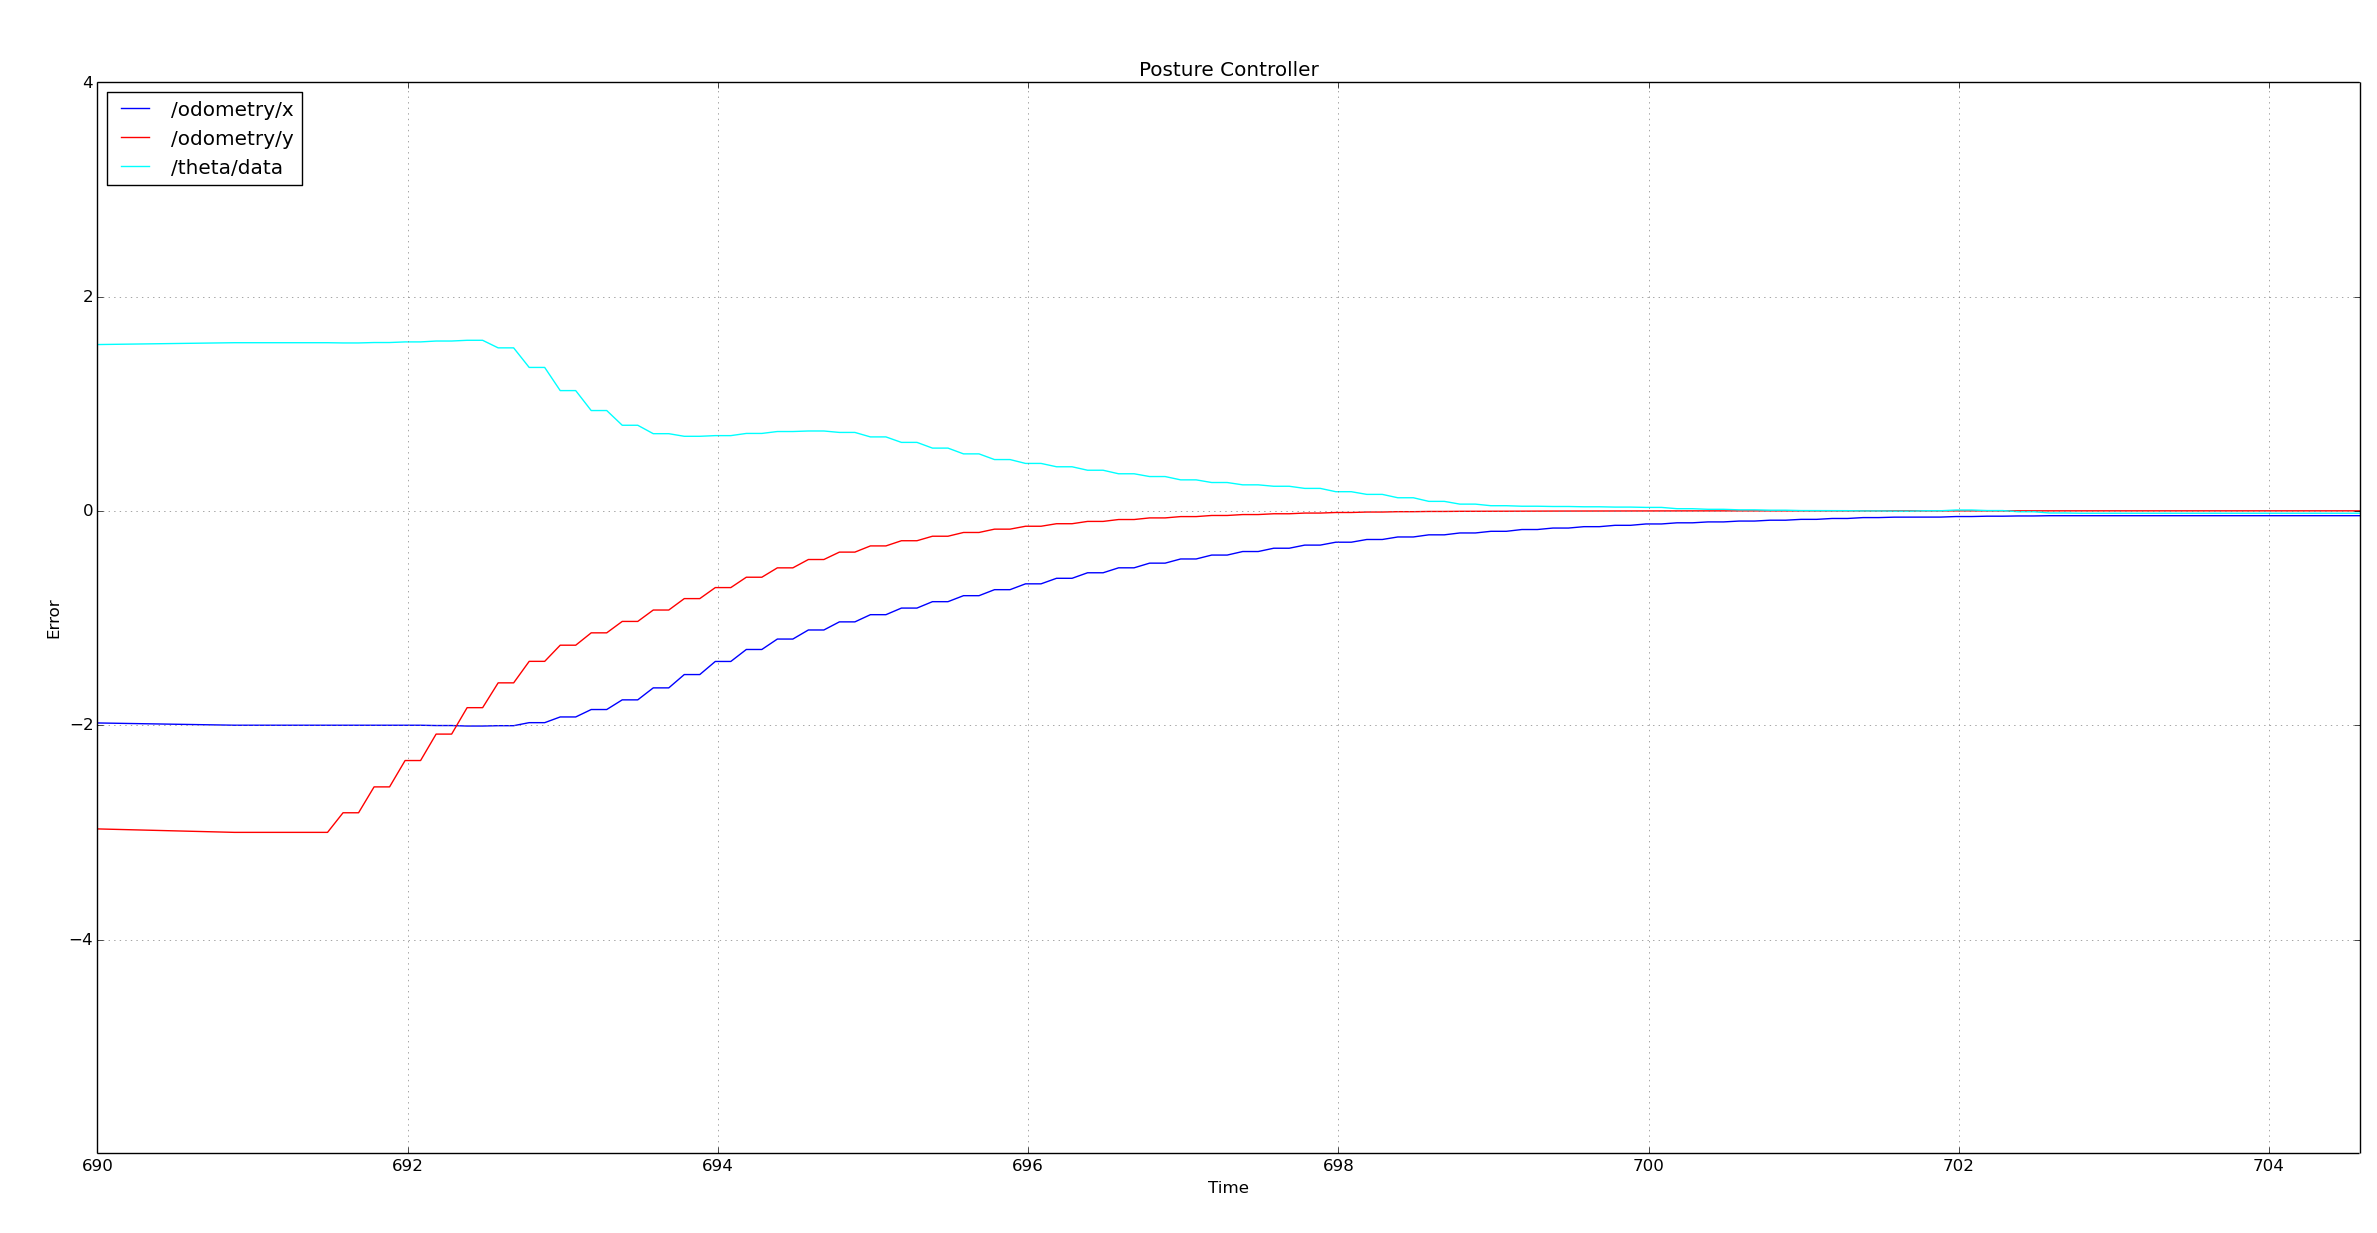
\includegraphics[width=1.1\textwidth]{rover2_rqt_plot93_high_error.png}
		\caption{ $x = -2,  y = -3,  \theta=\frac{\pi}{2}$}	
 		\label{fig:334322}
		\end{figure}

		We see that if we set very high errors (have the desired pose far away from where the robot is going), $\theta$ tends to be more unstable. We can also clearly here see the time samplings
		intervalls as small jumps in the graph. The fact that $\theta$ tends to be more unstable with more difficult odometric localizations is expected. The robot may need to turn suddenly in order
		to get into the right path. It would have been interesting to see if lower sampling time would have had a practical difference on the odometry and the controller.\\
		We noticed that the odometry always was off by something that looked like a scaling factor. In fact was this factor one of the first ting we started inversigeating by trial and error the first day
		(by mathematically making an expression for how much of 100\% speed for how long, one should drive in order to get to a position), but we did not get enough data to calculate it, because
		there was trouble with the rovers wifi. We assumed that the reason why the odometry was off must be because of that \textit{/est\_vel} were publishing wrong velocities. In order to
		compensate for the wrong/estimated velocities from the motordriver, we added a factor on the velocity like this;

		\begin{figure}[H]
		\centering
		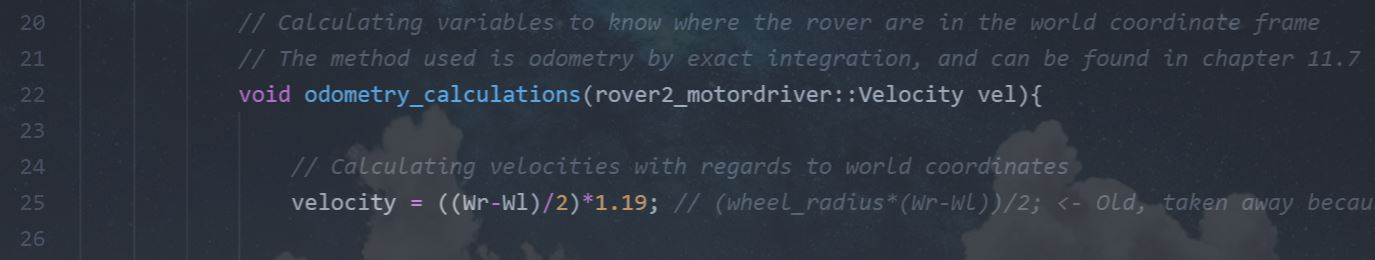
\includegraphics[width=1.1\textwidth]{snippet_adjustment_factor.JPG}
		%\caption{code}	
 		%\label{fig:3}
		\end{figure}
		It turned out 1.19 times the velocity gave us a pretty good result (cm tolerances), which confirmed our suspicion regarding the unknown constants in the motordriver.\\
		You can see two short videos of the robot driving with this new compensation in our github repository.


		So in the end we ended up with a good result, but some errors. It is worth noting that we implemented the odometry under the assumption of constant velocity inputs within the sampling
		intervall. That is definetly not the case because of the pid regulator in the motordriver, and that could explain some of the errors. We also came to the conclution that the motordriver sends
		out angular velocities in $m/s$, so we edited our code to compensate for that. We suspect that somewhere in the motordriver they do something wrong when trying to calculate velocities in
		$m/s$, and for further development of the system we would advise to calculate and send out $rad/s$, so that everything agrees with the formulas in the odometry by default.

		Another interesting experiment is based on the observation that the "2 4 1.3" regulator had higher speed going towards its goal, and therfore hit more in the middle of the $\pm0.05$ gap,
		while the "1 6 7" regulator was so slow that it stopped imidiatly after crossing the limit. It would have been interesting to lower the $\pm0.05$ limit and then try the "1 6 7" controller on
		longer distances, because it was a more "stable" controller.
		
		

\end{document}
